\subsection{Posizione del contesto nel prompt}

Un'ultima scelta, a valle di tutte quelle discusse finora, riguarda come assemblare nel prompt i frammenti
recuperati, ordinati per pertinenza: semplicemente concatenarli nell'ordine restituito dal reranking non è
necessariamente innocuo. Liu et al. \cite{liu2023lostmiddle} mostrano che un LLM non utilizza un contesto lungo in
modo uniforme: l'accuratezza nel reperire un'informazione specifica è più alta quando questa si trova all'inizio o
alla fine del contesto fornito, e cala sensibilmente quando si trova nel mezzo un andamento a U che gli autori
osservano persistere anche in modelli progettati esplicitamente per finestre di contesto lunghe, e che ricorda gli
effetti di primacy e recency studiati nella memoria umana(vedere la figura: \ref{fig:u-curve}).
\begin{figure}[H]
  \centering
  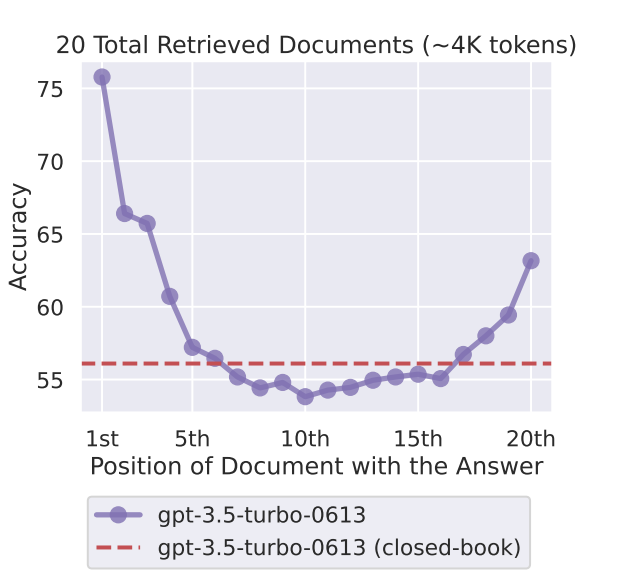
\includegraphics[width=0.5\textwidth]{assets/U-curve-diagram.png}
  \caption{La modifica della posizione delle informazioni rilevanti (in questo caso, la posizione del passaggio che risponde a una domanda in input) all'interno del contesto di input del modello linguistico produce una curva delle prestazioni a forma di U: i modelli sono più abili nell'utilizzare le informazioni rilevanti che compaiono all'inizio o alla fine del proprio contesto di input, e le prestazioni diminuiscono in modo significativo quando i modelli devono accedere e utilizzare informazioni situate nella parte centrale del proprio contesto di input. Fonte: Liu et al. \cite{liu2023lostmiddle} }
  \label{fig:u-curve}
\end{figure}

Per un sistema che costruisce il proprio contesto
unendo più frammenti recuperati, come quello di questo lavoro, questo risultato implica che l'ordine con cui i
frammenti vengono presentati al modello non è un dettaglio ininfluente quanto potrebbe sembrare a prima vista, specie
quando il numero di frammenti recuperati si avvicina al
limite superiore per cui l'effetto è stato osservato in letteratura.